\documentclass[twocolumn,showpacs,preprintnumbers,nofootinbib,prd,
superscriptaddress,10pt]{revtex4-2}

	%to make sure that pdflatex is used
\pdfoutput=1

\usepackage{amsmath,amssymb}
\usepackage{amsfonts}
\usepackage{mathtools}
\usepackage[normalem]{ulem}
\usepackage{textcomp}
\usepackage{enumitem}
\usepackage{bm}
\usepackage{bbm}
\usepackage{afterpage}
\usepackage{graphicx}
\graphicspath{{img/}} %setting img path
\usepackage{tensor}

\usepackage{tabularx}
\usepackage{longtable}
\usepackage{makecell}
\usepackage{multirow}
\usepackage{booktabs}


\usepackage{layouts}
\usepackage[usenames,dvipsnames]{xcolor}
\usepackage[utf8]{inputenc}
\usepackage{rotating}
\usepackage[bookmarks]{hyperref}
%\usepackage{ragged2e}
\usepackage{blindtext}
\usepackage{graphicx}
\usepackage{siunitx}
	\sisetup{output-decimal-marker={.}}
	
\usepackage{arydshln}

	%some math symbols
\newcommand{\R}{\mathbb{R}}
\newcommand{\N}{\mathbb{N}}
\DeclareMathOperator{\sign}{sign}
\renewcommand{\d}[1]{\ensuremath{\operatorname{d}\!{#1}}}
\newcommand{\dvol}[2]{\ensuremath{\operatorname{d}^{#2}\!{#1}}}
%argmin and argmax
\DeclareMathOperator*{\argmax}{arg\,max}
\DeclareMathOperator*{\argmin}{arg\,min}

\newcommand{\scalar}[2]{\langle #1|#2 \rangle}
\newcommand{\scalarnonorm}[2]{\langle #1|#2 \rangle_{\text{not normalized}}}
\newcommand{\rescalar}[2]{( #1 |#2 )}
\newcommand{\rescalarwide}[2]{\left( #1 \lvert #2 \right)}
\newcommand{\imscalar}[2]{[ #1|#2 ]}


% comments command
\newcommand{\stefano}[1]{{\textcolor{blue}{\texttt{SS: #1}} }}
\newcommand{\sarah}[1]{{\textcolor{red}{\texttt{SC: #1}} }}
\newcommand{\bhooshan}[1]{{\textcolor{cyan}{\texttt{BG: #1}} }}


\begin{document}

	%%%%%%%%%%%%%%%%%%%%%%%%%%%%%%%%% ABSTRACT
\begin{abstract}
	We introduce a novel method to generate a bank of gravitational-waveform templates of binary Black Hole (BBH) coalescences for matched-filter searches in LIGO, Virgo and Kagra data. Unlike the standard approach, our method relies on a numerical metric approximation of the distance between templates, which makes the template placement orders-of-magnitude faster than with existing techniques.
	Our method applies to a variety of different manifolds of signals and is particularly suitable for covering high-dimensional spaces, such as those associated with precessing and/or eccentric waveforms.
	We compare our method with the state-of-the-art stochastic placement code and find that our code slightly overcovers the space, while achieving similar efficiency in recovering signals. To demonstrate the capabilities of our code, we generate a bank for precessing Black Holes, a bank for intermediate-mass Black Holes with higher-order modes, and an eccentric bank, and show that they cover the space in a satisfactory way.
	Our publicly released code \texttt{mbank} will enable searches of high-dimensional regions of BBH signal space, hitherto unfeasible due to the prohibitive cost of bank generation.
\end{abstract}
	
	%%%%%%%%%%%%%%%%%%%%%%%%%%%%%%%%% TITLE
 %\title{Metric template placement for high dimensional regions of compact binary mergers}
 %\title{Fast metric-based template placement for gravitational-waves from novel compact binary mergers}
 %\title{Mbank: fast metric-based template banks for gravitational wave searches for exotic compact binaries}
 %\title{Template banks for exotic compact binaries}
 %\title{Template banks for novel compact binaries}
 \title{Gravitational-wave template banks for novel compact binaries}
	\author{Stefano \surname{Schmidt}}
		\email{s.schmidt@uu.nl}
        \affiliation{Nikhef, Science Park 105, 1098 XG, Amsterdam, The Netherlands}
        \affiliation{Institute for Gravitational and Subatomic Physics (GRASP),
Utrecht University, Princetonplein 1, 3584 CC Utrecht, The Netherlands}

	\author{Bhooshan \surname{Gadre}}
        \affiliation{Institute for Gravitational and Subatomic Physics (GRASP),
Utrecht University, Princetonplein 1, 3584 CC Utrecht, The Netherlands}
        
        %
	\author{Sarah \surname{Caudill}}
       \affiliation{Nikhef, Science Park 105, 1098 XG, Amsterdam, The Netherlands}
       \affiliation{Institute for Gravitational and Subatomic Physics (GRASP),
Utrecht University, Princetonplein 1, 3584 CC Utrecht, The Netherlands}
		\affiliation{Department of Physics, University of Massachusetts, Dartmouth, MA 02747, USA}
		\affiliation{Center for Scientific Computing and Visualization Research, University of Massachusetts, Dartmouth, MA 02747, USA}
	\maketitle

	%%%%%%%%%%%%%%%%%%%%%%%%%%%%%%%%% BODY 
\section{Introduction}

As gravitational-wave (GW) astronomy enters a mature state, the accessible parameter space of binary Black Hole (BBH) mergers in LIGO \cite{LIGOScientific:2014pky} and Virgo \cite{VIRGO:2014yos} data continues to grow. Besides standard aligned-spin GW searches for stellar-mass BBH mergers \cite{GWTC-1,GWTC-2,GWTC-2.1, GWTC-3}, there are GW searches targeting the parameter space of sub-solar mass Black Holes (BH) \cite{SSM_O2, SSM_O3a, PhysRevD.106.023024, Nitz:2021mzz}, primordial BHs \cite{PBH}, eccentric binaries \cite{PhysRevD.102.043005, PhysRevD.104.104016, Nitz:2019spj} and intermediate-mass BHs (IMBH) \cite{IMBH_O2, IMBH_O3, Chandra:2022ixv}. Moreover, there is a growing interest in GW searches for more complex binaries, such as those with precession \cite{PhysRevD.89.024010, Harry:2017weg, PhysRevD.102.041302, Indik:2016qky, Harry:2016ijz}, eccentricity \cite{LIGOScientific:2019dag, Ramos-Buades:2020eju, Wang:2021qsu, Nitz:2021mzz} or higher-order mode (HMs) content~\cite{CalderonBustillo:2015lrt, Harry:2017weg, Chandra_hom, 2021PhRvD.103b4042M}.

GW searches for signals from compact binary mergers traditionally utilize the method of matched-filtering with a template bank of model waveforms~\cite{Sathyaprakash:1991mt, Dhurandhar:1992mw, Owen:1998dk, Allen:2005fk, Babak:2006ty, Cokelaer:2007mv}.
An optimal template bank is composed by the smallest number of templates that guarantees that only a small fraction of GW signals are missed due to the discreteness of the template bank \cite{Prix:2007ks}.

One widely used approach to bank generation - the {\it stochastic} method \cite{Harry:2009ea, PhysRevD.80.104014, Ajith:2012mn} - consists of randomly scattering templates in a defined parameter space with a rejection technique \cite{DalCanton:2017ala, Mukherjee:2018yra, Indik:2016qky, Lenon:2021zac}. A proposed template is included in the bank only if its distance (or {\it mismatch}) with all the proposed templates in the bank is larger than the user-defined threshold.
While this approach has proven to be very powerful and generates template banks with very good coverage, it does not scale have a favourable scaling with the number of templates and, most importantly, with the number of dimensions of the parameter space.
Moreover, since it requires to generate many waveforms and to perform expensive match calculations, it can take up to months to generate a template bank.

As the volume of the parameter space for BBH searches grows due to including more complex binaries, the stochastic approach is struggling to produce template banks in a feasible amount of time.
Indeed so far, very few banks with precessing, eccentricity and/or HMs have been published \cite{Harry:2016ijz, Harry:2017weg} and they were  mostly intended as proof of principle, never been used in a real seach.
This poses the challenge of finding a viable alternative to template bank generation, which is able to deliver large template banks in a high dimensional parameter space, such as those associated to precession, eccentricity and HMs.

Revitalizing a pioneering line of research in bank generation \cite{owen_metric, Messenger:2008ta, Prix:2007ks, Brown:2012qf, Keppel:2013uma}, there has been recently an increasing attention on {\it metric template placement} \cite{Roy:2017oul, 2018cosp...42E2899R, Coogan:2022qxs, Hanna:2022zpk}.
Such methods rely on approximating the distance (or match) between two waveforms with a bilinear form, called metric.
Although the metric is only approximate, it allows for a faster template placing that may overcome some of the major limitations of the standard stochastic placement algorithm.

While the metric was first employed to place templates on a lattice \cite{owen_metric, Prix:2007ks}, {\it random} templates banks \cite{Messenger:2008ta} were introduced shortly afterwards.
Random template banks are designed to cover any point in space only with probability $\eta<1$. As they cover the space with random templates, they require the ability to effectively sample templates ``uniformly" across the parameter space.
The strength of the method relies on the fact that no distance between templates is computed, with great computational convenience.
While this may seem sub-optimal with respect to a lattice, in \cite{Messenger:2008ta, Allen:2022lqr, Allen:2021yuy} it is argued that in large number of dimension random template banks outperform even the best known lattice in terms of coverage (at a fixed number of templates), effectively beating the ``curse of dimensionality".

At this point it should be clear that random template banks are the ideal candidate to cover high dimensional spaces and for this reason, in this work we develop a novel algorithm to generate random template banks.
We derive an expression for the metric, which is suitable for generic precessing and/or HM waveforms, by dropping several symmetry assumptions that entered the standard metric computation. The metric is expressed in terms of the gradients of the waveform.
Our new metric expression, together with the random template placement algorithm, makes our method is particularly suited for dealing with high-dimensional ($>$ 4D) parameters, usually associated to precessing or eccentric searches.
Our method is implemented in an open-source, production-ready, python package \texttt{mbank}, available on GitHub\footnote{
\href{https://github.com/stefanoschmidt1995/mbank}{stefanoschmidt1995/mbank}.}
and on the PyPI repository\footnote{
The package is distributed under the name \texttt{\href{https://pypi.org/project/gw-mbank/}{gw-mbank}}.
}.

The rest of this paper is devoted to the presentation and description of our methods and package.
In Sec.~\ref{sec:methods} we present the details of our bank generation algorithm.
In Sec.~\ref{sec:validation} we assess the accuracy of our template placing method in all its parts.
We will also reproduce two banks available in the literature \cite{Harry:2017weg, Sakon:2022ibh} created with independent codes: this will be the topic of Sec.~\ref{sec:other_methods}.
To demonstrate the capabilities of \texttt{mbank}, in Sec.~\ref{sec:use_cases}, we present two large banks covering ``exotic" regions of parameter space: a precessing bank and an IMBH bank with HM content. We also present a study of the size of the precessing Neutron Start-Black Hole (NSBH) parameter space.
Finally, in Sec.~\ref{sec:conclusion} we conclude with some remarks on future prospects.

	%%%%%%%%%%%%%%%%%%%%%%%%%%%%%%%%%
\section{Methods} \label{sec:methods}

When searching for a BBH signal in GW data, it is customary to use a frequentist detection statistic~\cite{Creighton_book, Maggiore:2007ulw, Harry:2016ijz, Harry:2017weg}, which models the detector output to be composed of {\it gaussian} noise $n(t)$ and possibly a known GW signal $h(t)$.
Given some observed data $s(t)$, the detection statistic $\Lambda$ is a measure of the log probability ratio between the signal hypothesis $n+h$ and the noise hypothesis $n$:
\begin{equation}\label{eq:LL}
	\Lambda = \log\frac{p(s|n+h)}{p(s| n)}
\end{equation}
For a standard GW observatory such as LIGO and Virgo, the signal observed takes the following form:
\begin{equation}\label{eq:signal_model}
	h(t) = F_+(\delta, \alpha, \Psi) h_+(t;\theta) + F_\times(\delta, \alpha, \Psi) h_\times(t;\theta)
\end{equation}

The functions $F_+, F_\times$, also called Antenna Patterns, denote the interferometer response to the two polarizations of a GW. They depend on the sky location, parameterized by right ascension $\alpha$ and declination $\delta$, and on the polarization angle $\Psi$. 
For a BBH system, the two polarizations $h_+, h_\times$ depend on two BH masses ($m_1$, $m_2$), two 3-dimensional spins ($\mathbf{s}_1$, $\mathbf{s}_2$), the inclination angle $\iota$, the reference phase $\phi$, the luminosity distance of the source $D_L$, the eccentricity $e$ of the orbit and the mean periastron anomaly $a$ \cite{Sathyaprakash_2009}.

Under the assumption of {\it gaussian noise}, we can write down an explicit model for the likelihood and, after maximising over an overall amplitude factor, Eq.~\eqref{eq:LL} becomes \cite{Creighton_book, Maggiore:2007ulw, Harry:2016ijz}:
\begin{equation}\label{eq:LL_gauss}
	\Lambda = \frac{\left(\Re\scalar{s}{h}\right)^2}{\scalar{h}{h}} = \rescalar{s}{\hat{h}}^2
\end{equation}
where we introduced a {\it complex} scalar product between two signals $a$, $b$:
\begin{equation} \label{eq:scalar_product}
	\scalar{a}{b} = 4 \int_{f_\text{min}}^{f_\text{max}} \!\!\!\! \d{f} \; \frac{\tilde{a}^*(f) \tilde{b}(f)}{S_n(f)}
\end{equation}
where the integral extends in a suitable frequency range $[f_\text{min}, f_\text{max}]$.
In this context, $S_n(f)$ is the frequency domain autocorrelation function of the noise, also called Power Spectral Density (PSD) and $\tilde{\phantom{a}}$ denotes the Fourier transform.
For ease of notation, we define ${\rescalar{a}{b} = \Re\scalar{a}{b}}$ and ${\hat{a} = \frac{a}{\rescalar{a}{a}}}$.

For any given observation time, a search aims to {\it maximize} the detection statistics $\Lambda$ with respect to all the parameters of the signal model: this maximized quantity is also called signal-to-noise ratio (SNR).
Depending on symmetry assumptions on the polarizations, one is able to maximize analytically over some (nuisance) parameters.
For the other quantities, a brute force approach is required, where the maximized $\Lambda$ is evaluated at each time on a large set of signal models, called a {\it template bank} \cite{PhysRevD.77.104017, Mukherjee:2018yra}.
This procedure is called {\it matched filtering} and it has been implemented successfully by several pipelines to search for GW signals \cite{Privitera:2013xza, Usman:2015kfa, Capano:2016dsf, PhysRevD.95.042001, gstlal_paper2, Aubin:2020goo, Chu:2020pjv}.

For a non-precessing signal, it holds $\tilde{h}_+ \propto i\tilde{h}_\times$ and the maximization of Eq.~\eqref{eq:LL_gauss} over the nuisance parameters yields:
\begin{equation}\label{eq:std_snr}
	\max \Lambda = \lVert \scalar{s}{\hat{h}_+} \rVert^2 = \rescalar{s}{\hat{h}_+}^2 + \rescalar{s}{\hat{h}_\times}^2
\end{equation}
In this simple case, $\max\Lambda$ only depends on the two BH masses $m_1, m_2$ and the two z-components of the spins $s_{1z}, s_{2z}$ (4 quantities).

For the general case, where no particular symmetry is available, one obtains a different expression:
\begin{equation}\label{eq:symphony_snr}
	\max \Lambda = \frac{ \rescalar{s}{\hat{h}_+}^2 + \rescalar{s}{\hat{h}_\times}^2 -2\rescalar{\hat{h}_+}{\hat{h}_\times}\rescalar{s}{\hat{h}_\times}\rescalar{s}{\hat{h}_+}}{1- \rescalar{\hat{h}_+}{\hat{h}_\times}^2}
\end{equation}
In this case, $\max\Lambda$ depends on 12 parameters: they are the two BH masses $m_1, m_2$, the two three-dimensional spins $\mathbf{s}_1$, $\mathbf{s}_2$, the inclination angle $\iota$, the reference phase $\phi$ and the eccentricity parameters $e, a$.
Unlike the non-precessing case, the analytical maximisation removed the dependence of $\Lambda$ on fewer parameters.F
Depending on the scope of a matched-filtering search, a pipeline can use either Eq.~\eqref{eq:std_snr} or Eq.~\eqref{eq:symphony_snr} to filter the interferometer data with templates.

For the purpose of template placement, it is useful to think of the parameter space of BBH signals as a D-dimensional manifold $\mathcal{B}_D$, embedded in a large 12 dimensional manifold $\mathcal{B}$. Each point of the manifold corresponds to a GW signal. The number of dimensions $D$ depends on the BBH variables under consideration.
As the parameters that do not enter the interesting space can be freely neglected (i.e. set to $0$ or to a meaningful default value), the manifold $\mathcal{B}_D$ is effectively a lower dimensional {\it projection} of the large manifold $\mathcal{B}$.

To place templates on $\mathcal{B}_D$, it is standard to equip the manifold with a distance (called {\it mismatch}), which also naturally defines a volume element at every point in space. The volume element defines the ``uniform" probability distribution according to the metric.
A random template bank will be populated by templates drawn from such distribution, until a certain coverage is reached. For this reason, our primary concern is to sample from the manifold and to check for coverage. To effectively do so, we rely on the three steps below:
\begin{enumerate}
	\item Construction of a metric approximation of the match between templates. This makes $\mathcal{B}_D$ a Riemannian manifold with a volume element
	\item Training of a normalizing flow model to sample from the manifold. 
	\item Placing the templates by sampling from the normalizing flow model and checking for coverage.
\end{enumerate}
The rest of this section details the steps above.

\subsection{The metric} \label{sec:metric}

W define a metric on the manifold $\mathcal{B}_D$: this will provide a a fast-to-compute approximation to the {\it mismatch} (distance) between templates and an estimation to the volume element of each point in the space.

Given two points of the manifold $\theta_1,\theta_2$, we define the overlap $\mathcal{O}(\theta_1,\theta_2, t)$ between normalized templates as:
\begin{widetext}
	\begin{align}\label{eq:overlap}
		\mathcal{O}(\theta_1,\theta_2, t) &= \frac{1}{1- \hat{h}_{+\times}(\theta_2)^2} 
		\biggl\{ \rescalarwide{\hat{h}_+(\theta_1)e^{i ft}}{\hat{h}_+(\theta_2)}^2 + \rescalarwide{\hat{h}_+(\theta_1)e^{i ft}}{\hat{h}_\times(\theta_2)}^2 \nonumber \\
		& -2h_{+\times}(\theta_2)\rescalarwide{\hat{h}_+(\theta_1)e^{i ft}}{\hat{h}_\times(\theta_2)}\rescalarwide{\hat{h}_+(\theta_1)e^{i ft}}{\hat{h}_+(\theta_2)} \biggl\}
	\end{align}
\end{widetext}
where $\hat{h}_+(\theta)e^{i ft}$ is the plus polarization $\hat{h}_+(\theta)$ translated by a constant time $t$ and $\hat{h}_{+\times}(\theta) = \rescalar{\hat{h}_+(\theta)}{\hat{h}_\times(\theta)}$.
The overlap amounts to the fraction of SNR recovered when filtering a signal $s=h_+(\theta_1)$ with a template evaluated at a point $\theta_2$ (see also Eq.~\eqref{eq:symphony_snr}).
In the case of a non-precessing search, it holds $h_{+\times} = 0$ and $\tilde{h}_\times = i \tilde{h}_+$, hence the overlap simplifies to:
\begin{equation}\label{eq:overlap_NP}
\mathcal{O}(\theta_1,\theta_2, t) = \left|\scalar{\hat{h}_+(\theta_1)e^{i ft}}{\hat{h}_+(\theta_2)} \right|^2
\end{equation}
All the literature available \cite{owen_metric, Messenger:2008ta, Prix:2007ks, Brown:2012qf, Roy:2017oul, Coogan:2022qxs, Hanna:2022zpk} relies on the latter expression to derive the metric, addressing only the non-precessing case, whereas we tackle the most general case.

We can maximize the overlap Eq.~\eqref{eq:overlap} with respect to time to obtain the match $\mathcal{M}(\theta_1,\theta_2)$ between templates evaluated at different points of the manifold:
\begin{equation}\label{eq:match}
	\mathcal{M}(\theta_1,\theta_2) = \max_t \mathcal{O}(\theta_1,\theta_2, t). \\
\end{equation}
%
The match has values in $[0,1]$ and trivially $\mathcal{M}(\theta,\theta) = 1$.

We use the match to introduce a {\it distance} $d$ \footnote{
From a strict geometrical point of view, this is not a distance since it does neither symmetry nor triangular inequality. However, this does not affect its effectiveness in measuring the ``dissimilarity" between two waveforms and it will be used regardless.}
between two points on the D-manifold $\mathcal{B}_D$:
\begin{align}\label{eq:distance}
	d^2(\theta_1,\theta_2) \vcentcolon= 1 - \mathcal{M}(\theta_1,\theta_2)
\end{align}
The distance $d$ can then by approximated locally by a bilinear form $d_M$:
\begin{align}\label{eq:metric_definition}
	d_M^2(\theta_1,\theta_2) \vcentcolon= M_{ij}(\theta) \Delta\theta_i \Delta\theta_j \simeq 1 - \mathcal{M}(\theta_1,\theta_2)
\end{align}
The bilinear form $d_M$ is represented by a D-dimensional square matrix $M_{ij}(\theta)$, defined at each point of the manifold.

Following a standard practice, we identify $M_{ij}(\theta)$ to be the quadratic term of the Taylor expansion of $d_M(\theta+\Delta\theta,\theta)$ around $\Delta\theta\simeq 0$:
\begin{equation}\label{eq:metric_expression}
	M_{ij}(\theta) = - \frac{1}{2} \left( H_{ij} - \frac{H_{ti}H_{tj}}{H_{tt}} \right)
\end{equation}
where $H(\theta)$ is the Hessian of the overlap Eq.~\eqref{eq:overlap}, a $D+1$ square matrix.
Note that the metric is positive definite. A convenient expression of the $H$ in terms of the gradients of the waveform is presented in App.~\ref{app:metric}, the full expression being in Eqs.~\eqref{eq:H_tt_grad}-\eqref{eq:H_ij_grad}.
While identifying the metric with the Hessian is well motivated and yields reliable results, other definitions for $M_{ij}$ are available: this is briefly discussed in App.~\ref{app:metric_definition}.

For most of the waveform models available, the gradients can be evaluated with finite difference methods. For a limited number of machine-learning based models \cite{Khan:2020fso, PhysRevD.103.043020, ML_wf_model, Tissino:2022thn}, such gradients are available analytically.

Equipped with the metric from Eq.~\eqref{eq:metric_expression}, the manifold $\mathcal{B}_D$ becomes a Riemannian manifold with line element:
\begin{equation}\label{eq:line_element}
	\d{s^2} = M_{ij}(\theta) \d{\theta_i} \d{\theta_j}.
\end{equation}
We can then use standard results from differential geometry to compute distances and volumes. In particular, the volume of a subset $\mathcal{T}$ of the manifold can be computed as:
\begin{equation}\label{eq:volume_tile}
	\text{Vol}(\mathcal{T}) = \int_\mathcal{T} \dvol{\theta}{D} \; \sqrt{|\text{det}M(\theta)|}.
\end{equation}
where $\text{det}M(\theta)$ is the determinant of the matrix $M_{ij}(\theta)$.
%
Moreover, we introduce the uniform probability measure, such that $p(V) \propto \text{Vol}(V)$ for any $V\subseteq \mathcal{B}_D$. The measure has the following probability distribution function (PDF):
\begin{equation}\label{eq:pdf_uniform}
	p(\theta) \propto \sqrt{|\text{det}M(\theta)|}.
\end{equation}
Samples from the uniform distribution tend to have an ``uniform" (i.e. constant) spacing, computed with the metric distance. Thanks to this feature, the uniform distribution is a natural candidate to draw template proposals from.

\subsection{Sampling from the manifold} \label{sec:normalizing_flow}

To generate a random template bank, we are interested in sampling from the manifold $\mathcal{B}_D$ from the PDF Eq.~\eqref{eq:pdf_uniform}.
The easiest way to obtain a number of samples is by means of a Markov Chain Montecarlo. However, this turns out to be unfeasibly expensive, since to obtain a single sample, the metric must be evaluated tens of times, which is too slow even for a moderately small number of dimensions.
To overcome this problem, we introduce a {\it normalizing flow} model. Once trained, it produces high quality samples from Eq.~\eqref{eq:pdf_uniform} in a small amount of time, effectively providing templates to populate a random template bank.

A normalizing flow model \cite{norm_flow, nflows_paper, Kobyzev_2021, Papamakarios_thesis} is a machine learning model widely used to reproduce and/or parametrize complicated probability distributions.
Mathematically, a flow is an {\it invertible} parametric function $\phi_W$ which is trained to map samples $\theta$ from an arbitrary probability distribution $p(\theta)$ to samples $\mathbf{x}$ from a multivariate standard normal distribution.
The parameters $W$ of the flow are set in such a way that:
\begin{equation}
	\mathbf{x} = \phi_W(\theta) \sim \mathcal{N}(\mathbf{x}|0,\mathbf{1}) \;\;\; \text{if} \;\;\;  \theta \sim p(\theta)
\end{equation}
%
In other words, a normalizing flow defines a parametric representation of a generic probability distribution $p(\theta)$, obtained by change of variables
\begin{equation}\label{eq:p_flow}
	p^\text{flow}_W(\theta) = \mathcal{N}(\phi_W(\theta)|0,\mathbf{1}) \; |\text{det} J_{\phi_W}(\theta)|
\end{equation}
where $J_{\phi_W}$ is the Jacobian of the flow transformation $\phi_W$.
Sampling from $p^\text{flow}_W$ can then be easily done by sampling $\mathbf{x} \sim \mathcal{N}(\mathbf{x}|0,\mathbf{1})$ and obtaining $\theta$ from the inverse flow transformation: $\theta = \phi_W^{-1}(\mathbf{x})$.
Thus, the normalizing flow model makes tractable the problem of sampling from the target distribution and at the same time of evaluating a PDF at each point.


The flow transformation $\phi_W$ is built by {\it composing} $n_\text{layers}$ simple (invertible) transformations, each called layers. Of course, depending on the application, a variety of layers are available in the literature. We choose to build a layer by concatenating a linear transformation and a Masked Auto-regressive Layer \cite{MADE, MAF,MAF_bis} with $n_\text{hidden}$ hidden features.
A Masked Auto-regressive Layer implements the following transformation:
\begin{equation}
	T_{MADE}(\theta) = a(\theta)\theta+b(\theta)
\end{equation}
where the coefficients $a(\theta), b(\theta)$ are computed by a (Masked) Autoencoder with $n_\text{hidden}$ hidden features.

To deal with a probability distribution bounded in the rectangle $[\theta_\text{min}, \theta_\text{max}]$, we employ the following transformation $T_0(\theta)$ as the first layer of the flow:
\begin{equation}
	T_0(\theta) = 0.5 \log \frac{1 + y}{1 - y} \;\;\; \text{with} \;\;\; y = \frac{2\theta - \theta_\text{min} - \theta_\text{max}}{\theta_\text{max}- \theta_\text{min}}
\end{equation}
where the fraction above is intended as elementwise division.\footnote{
Note that the inverse $T_0^{-1}$ of the transformation takes a simple form: $\frac{1}{2} [\text{Tanh}(T_0(\theta))(\theta_\text{max} - \theta_\text{min})+\theta_\text{max}+ \theta_\text{min}]$, where again the multiplication is intended as elementwise.
}


The flow probability distribution $p^\text{flow}_W(\theta)$ is trained to closely reproduce a given probability distribution $p^\text{target}(\theta)$.
During the training, the weights $W$ of the flow are set by minimizing a loss function $\mathcal{L}_\phi(W)$, which measures the discrepancy between $p^\text{target}$ and $p^\text{flow}_W$. The minimization is performed by gradient descent.


Depending on the nature of the data, several loss functions are available.
If {\it samples} from the target distribution are available, the loss function is defined as the forward Kullback–Leibler (KL) divergence between the target distribution $p^\text{target}(\theta)$ and the one defined by the flow Eq.~\eqref{eq:p_flow}:
\begin{align}
	\mathcal{L}^{KL}_\phi(W) = - \mathbb{E}_{p^\text{target}(\theta)} [\log p^\text{flow}_W] + \text{const.}
\end{align}
where the expected vaue is computed using empirical samples from $p^\text{target}(\theta)$ to provide a Monte-Carlo estimation of the loss function.

In our situation however, we do not have access to such samples (indeed, we are training the flow precisely to avoid sampling!) but we are only able to evaluate $p^\text{target}$ as in Eq.~\eqref{eq:pdf_uniform}.
For this reason, we treat the training as a regression problem and we use the following loss function:
%
\begin{align}
	\mathcal{L}_\phi(W) = \frac{1}{N} \sum_{i=1}^N \left(\log p^\text{flow}_W(\theta_i) - \log p^\text{target}(\theta_i) + C \right)^2
\end{align}
%
where the sum runs on a dataset of $N$ points $\{(\theta_i, \sqrt{|\text{det}M(\theta_i)|})\}_{i=1}^N$.

The values of $\theta_i$ are obtained by sampling the masses $m_1, m_2$ from
\begin{equation}
	p(\mathcal{M}_c, \eta) \propto \mathcal{M}_c^{10/3} \eta^{8/5}
\end{equation}
where $\mathcal{M}_c = \frac{(m_1m_2)^{3/5}}{(m_1+m_2)^{1/5}}$ is called the chirp mass and $\eta = \frac{m_1m_2}{(m_1+m_2)^2}$ is the symmetric mass ratio.
All the other quantities are sampled from a uniform distribution.
Our choice ensures that more samples are present at low chirp mass, which is where the metric tends to have larger values due to longer waveforms (at constant starting frequency).

The constant $C$ is a {\it trainable} constant that sets an overall shift to the log PDF predicted by the flow. The scaling can be beneficial to adjust the values of $\sqrt{|\text{det}M(\theta)|}$, potentially unconstrained, to a scale which is easier to learn by the normalizing flow.
Some heuristics suggests to initialize the constant to the $90^\text{th}$ percentile of the values $\log \sqrt{|\text{det}M(\theta)|}$ stored in the dataset.

\subsection{Random template placing} \label{sec:template_placing}

As is common, the input parameter controlling the average spacing and number of templates is the {\it minimum match} $MM$. It is defined as the minimum tolerable match that a random signal (inside the relevant space) must have with its nearest templates of the bank. It comes as input to virtually any template placement method in the literature.

To generate our random template bank, following \cite{Messenger:2008ta}, we add random templates to the bank until a satisfactory coverage is achieved. The covergae is checked using a procedure that closely matches \cite{Coogan:2022qxs}.
The templates are sampled from the normalizing flow Eq.~\eqref{eq:p_flow}, which, as discussed above, is trained to target the Eq.~\eqref{eq:pdf_uniform}. This choice makes sure that the templates are sampled as ``uniformly as possible" around the manifold.
One point of the space $\theta$ is said to be {\it covered} by the bank if there is at least one template $\theta_T$ in the bank, whose squared metric distance (mismatch) Eq.~\eqref{eq:metric_definition} is at at most $1 - MM$, i.e. $d_M(\theta, \theta_T)<1 - MM$.
The covering fraction $\hat{\eta}$ of a given region $\mathcal{T}$ of the parameter space is then defined as the fraction of volume covered by the bank:
\begin{equation}\label{eq:coverage}
	\hat{\eta}(\mathcal{T}) = \frac{1}{\text{Vol}(\mathcal{T})} \int_\mathcal{T} \dvol{\theta}{D} \; \sqrt{|\text{det}M(\theta_i)|} \; c(\theta).
\end{equation}
where $c(\theta)$ is an indicator function:
\begin{equation}\label{eq:coverage}
	c(\theta) = \left\{
                \begin{array}{ll}
                  1 \;\; \text{if $\theta$ is covered by the bank}\\
                  0 \;\; \text{otherwise}
                \end{array}
              \right.
\end{equation}

We do not require that the space is fully covered but we only require that it is covered with probability $\eta$. This means that we terminate the bank construction when the covering fraction $\hat{\eta} \geq \eta$.
To provide a sensible estimate of the covering fraction $\hat{\eta}$, we perform a Monte Carlo estimation of the integral Eq.~\eqref{eq:coverage}, using importance sampling:
\begin{equation}\label{eq:coverage}
	\hat{\eta}(\mathcal{T}) \simeq \frac{1}{\sum_i w_i} \sum_i c(\theta_i) w_i 
\end{equation}
where the $N_\text{livepoints}$ samples $\theta_i \sim p^\text{flow}$ are samples from the normalizing flow and are called {\it livepoints}.
The weigths $w_i = \frac{\sqrt{|\text{det}M(\theta_i)|}}{p^\text{flow}(\theta_i)}$ take into account that, even if we are sampling from the flow, we want to compute the coverage of the space with volume element $\sqrt{|\text{det}M(\theta_i)|}$.

In practice, while the templates are being added to the banks, the distance between each livepoint is computed: if the i-th livepoint is close enough to the newly added template, it will be removed from the set of livepoints and a running estimate of $\hat{\eta}(\mathcal{T})$ will be updated with $w_i$.
The estimation of the covering fraction $\hat{\eta}$ has standard deviation \cite[App. A]{Coogan:2022qxs}:
\begin{equation}\label{eq:variance_coverage}
	\sigma_{\hat{\eta}} = \sqrt{\frac{\eta(1-\eta)}{N_\text{livepoints}-1}}
\end{equation}
which suggests to use a large number of livepoints for better estimation of $\hat{\eta}$.
In \cite{Coogan:2022qxs}, the authors typically chooses $\eta = 0.9$ and $N_\text{livepoints} = 2000$.

Since the method does not check for distances between templates, it can overcover the space (as reported also in \cite{Messenger:2008ta, Coogan:2022qxs}), especially in low number of dimensions.
Despite this, it is very fast and provides a reliable bank at a cheap computational and memory cost.
Moreover, as argued in \cite{Messenger:2008ta, Allen:2021yuy, Allen:2022lqr}, for a large number of dimensions, the banks generated by the random method provide close to optimal performance.

As a final remark, we note that for the purpose of computating the covering fraction, the templates do not need to be stored. Hence, the algorithm doesn't require much memory or computing time to measure the number of templates in a given template bank.
This enables several studies of the number of templates that are required to cover a particular region of the parameter space, giving invaluable information needed to plan a GW search. An example of this will be reported in Sec.~\ref{sec:NSBH}

	%%%%%%%%%%%%%%%%%%%%%%%%%%%%%%%%%
\section{Validation} \label{sec:validation}

\subsection{Normalizing flow validation} \label{sec:flow_validation}

\subsection{Template placement performance} \label{sec:template_placement}

\section{Comparison with other bank generation codes} \label{sec:other_methods}

\subsection{A non spinning HM bank} \label{sec:HM_comparison}

\subsection{An all sky bank} \label{sec:all_sky_comparison}

\section{Use cases} \label{sec:use_cases}

\subsection{Studying the precessing NSBH parameter space} \label{sec:NSBH}

\subsection{A precessing bank} \label{sec:precessing_bank}

\subsection{A spinning HM bank} \label{sec:HM_spinning_bank}

\section{Final remarks and future prospects} \label{sec:conclusion}


	%%%%%%%%%%%%%%%%%%%%%%%%%%%%%%%%% ACKNOWLEDGMENTS
        \begin{acknowledgments}
		S.S., B.G., and S.C. are supported by the research program of the Netherlands Organization for Scientific Research (NWO).
		The authors are grateful for computational resources provided by the LIGO Laboratory and supported by the National Science Foundation Grants No. PHY-0757058 and No. PHY-0823459. This material is based upon work supported by NSF’s LIGO Laboratory which is a major facility fully funded by the National Science Foundation.
%		We thank Melissa Lopez Portilla, Aaron Zimmerman and Keith Riles for precious comments.
        \end{acknowledgments}

	%%%%%%%%%%%%%%%%%%%%%%%%%%%%%%%%% APPENDIX
%\newpage
\appendix

\section{Details of the metric computation}\label{app:metric}

In this Appendix we report the details of the derivation of the Eq.~\eqref{eq:metric_expression}, as well as the computation of the Hessian $H$ of the overlap Eq.~\eqref{eq:overlap} in terms of the gradients of the waveform $h(\theta)$. 
In what follows, we define $\rescalar{h_1}{h_2}$ and $\imscalar{h_1}{h_2}$ to be respectively the real and imaginary part of $\scalar{h_1}{h_2}$.

We begin by expanding the quantity $\mathcal{M}(\theta+\Delta\theta,\theta )$ for $\Delta\theta$ around $0$. Since the $\mathcal{M}(\theta+\Delta\theta,\theta )$ has a maximum for $\Delta\theta = 0$, the leading term is quadratic in $\Delta\theta$.
We obtain:
\begin{align} \label{eq:metric_derivation}
	&\mathcal{M}(\theta+\Delta\theta,\theta ) = \max_{\Delta t} \mathcal{O}(\theta + \Delta\theta, \theta, \Delta t) \nonumber\\
	& =	\max_{\Delta t} \left\{ 1+ \frac{1}{2}\left[ \partial_{ij}\mathcal{O} \Delta\theta_i \Delta\theta_j + 2  \partial_{it}\mathcal{O} \Delta\theta_i \Delta t + \partial_{tt}\mathcal{O} (\Delta t)^2 \right] \right\}  \nonumber \\
	&= 1 + \frac{1}{2}\left[ \partial_{ij}\mathcal{O} - \frac{\partial_{it}\mathcal{O} \partial_{jt}\mathcal{O}}{\partial_{tt}\mathcal{O}}\right] \Delta\theta_i \Delta\theta_j
\end{align}
where all the derivatives are evaluated at ${\Delta\theta = \Delta t = 0}$ and the explicit time maximization yields
${\Delta t = -\frac{\partial_{it}\mathcal{O} \Delta\theta_i}{\partial_{tt}\mathcal{O}}}$.

From the above Eq.~\eqref{eq:metric_derivation}, we can read the expression for the metric in Eq.~\eqref{eq:metric_expression} recognizing in the derivatives $\partial\partial\mathcal{O}|_{\Delta\theta, \Delta t = 0}$ the components of the Hessian matrix $H$ of the overlap.

We now compute the Hessian of the overlap as a function of the gradients of the {\it normalized} waveforms. For notational convenience, we set $h_+(\theta_1)e^{ift} = s$, we drop any dependence on $\theta_2$ and we understand $\mu = {i, t}$.
We have:
\begin{align}\label{eq:overlap_grads}
	\partial_{\mu} \mathcal{O} &= \frac{1}{\mathcal{O}} \frac{1}{1-\hat{h}^2_{+\times}}
	\left[
	\rescalar{\partial_\mu\hat{s}}{\hat{h}_+}\rescalar{\hat{s}}{\hat{h}_+} 
	+ \rescalar{\partial_\mu\hat{s}}{\hat{h}_\times}\rescalar{\hat{s}}{\hat{h}_\times} \right. \nonumber \\
	&\left. - \rescalar{\partial_\mu\hat{s}}{\hat{h}_+}\rescalar{\hat{s}}{\hat{h}_\times}h_{+\times}
	- \rescalar{\partial_\mu\hat{s}}{\hat{h}_\times}\rescalar{\hat{s}}{\hat{h}_+}h_{+\times}
	\right]
\end{align}
Differentiating another time, after some rearrangements, we get:
\begin{align}
H_{tt} &= - \rescalar{\hat{h}_+}{\hat{h}_+f^2}
			+ \frac{1}{1-\hat{h}^2_{+\times}} \imscalar{\hat{h}_\times}{\hat{h}_+f}^2 \label{eq:H_tt}\\
H_{ti} &= \imscalar{\hat{h}_+}{\partial_i \hat{h}_+f}
			- \frac{1}{1-\hat{h}^2_{+\times}} \rescalar{\hat{h}_\times}{\partial_i\hat{h}_+} \imscalar{\hat{h}_\times}{\hat{h}_+f} \label{eq:H_ti}\\
H_{ij} &= \rescalar{\hat{h}_+}{\partial_i\partial_j\hat{h}_+}
			+ \frac{1}{1-\hat{h}^2_{+\times}} \rescalar{\hat{h}_\times}{\partial_i\hat{h}_+} \rescalar{\hat{h}_\times}{\partial_j\hat{h}_+} \label{eq:H_ij}
\end{align}

To move further, we express a normalized waveform derivatives in terms of the un-normalized ones:
\begin{align*}
	\bullet&\quad \partial_i \scalar{h}{h} = \scalar{\partial_i h}{h}+ \scalar{h}{\partial_i h} = 2 \rescalar{h}{\partial_i h} \\
	\bullet&\quad \partial_i \hat{h} =\frac{1}{\rescalar{h}{h}^{3/2}} \left[ \rescalar{h}{h}\partial_i h -  \rescalar{h}{\partial_i h} h \right]
	\\
	\bullet &\quad \partial_t \hat{h} = i f \hat{h} = i f \frac{h}{\rescalar{h}{h}^{1/2}} \\
	\bullet &\quad \partial_i \partial_j \hat{h} = \frac{1}{\rescalar{h}{h}^{1/2}} \partial_{ij}h 	+3 \frac{1}{\rescalar{h}{h}^{5/2}} \rescalar{h}{\partial_i h}\rescalar{h}{\partial_j h}h \\
	&- \frac{1}{\rescalar{h}{h}^{3/2}} \left[\rescalar{h}{ \partial_{ij} h} h + \rescalar{\partial_i h}{\partial_j h}  h
		+2\rescalar{h}{\partial_{(i} h} \partial_{j)} h \right]
\end{align*}
where $A_{(ij)} = \frac{1}{2}(A_{ij}+A_{ji})$ denotes symmetrization.

Plugging this into the equations~\eqref{eq:H_tt}-\eqref{eq:H_ij}, we get:
\begin{widetext}
\begin{align}
	H_{tt} &= - \frac{1}{h_{++}} \rescalar{h_+}{f^2 {h_+}}
		+ \frac{1}{1-\hat{h}^2_{+\times}} \frac{1}{h_{++}h_{\times\times}} \imscalar{{h_\times}}{f{h_+}}^2 \label{eq:H_tt_grad} \\
	H_{ti} &= - \frac{1}{h_{++}} \rescalar{h_+}{f \partial_i h_+}
		- \frac{1}{1-\hat{h}^2_{+\times}} \frac{1}{h_{++}h_{\times\times}} \imscalar{{h_\times}}{f{h_+}} \rescalar{{h_\times}}{\partial_i h_+}
		+ \frac{\hat{h}_{+\times}}{1-\hat{h}^2_{+\times}} \frac{1}{h^{3/2}_{++}h^{1/2}_{\times\times}}
			\imscalar{{h_\times}}{f{h_+}} \rescalar{{h_+}}{\partial_i h_+} \label{eq:H_ti_grad}\\
	H_{ij} &= - \frac{1}{h_{++}} \rescalar{\partial_i h_+}{\partial_j h_+}
		+ \frac{1}{1-\hat{h}^2_{+\times}} \frac{1}{h^2_{++}} \rescalar{h_+}{\partial_i {h_+}} \rescalar{{h_+}}{\partial_j {h_+}}
		+ \frac{1}{1-\hat{h}^2_{+\times}} \frac{1}{h_{++}h_{\times\times}} \rescalar{h_\times}{\partial_i {h_+}} \rescalar{{h_\times}}{\partial_j {h_+}} \nonumber \\
		& - \frac{2 \hat{h}_{+\times}}{1-\hat{h}^2_{+\times}} \frac{1}{h^{3/2}_{++}h^{1/2}_{\times\times}}
		\rescalar{h_\times}{\partial_{(i} {h_+}} \rescalar{{h_+}}{\partial_{j)} {h_+}} \label{eq:H_ij_grad}
%
%
%
%	\frac{1}{\rescalar{h}{h}^{2}}  \imscalar{h}{\partial_i {h}} \rescalar{{h}}{{h}f} +\rescalar{h}{\partial_i {h}} \imscalar{h}{hf}
%	&- \frac{1}{\rescalar{h}{h}} \imscalar{h}{\partial_i{h} f } \label{eq:H_ti_grad} \\
	%H_{ij} &=  \frac{1}{\rescalar{h}{h}^{2}} \Big\{ \rescalar{h}{\partial_i {h}} \rescalar{{h}}{\partial_j {h}} +\imscalar{h}{\partial_i {h}} \imscalar{h}{\partial_j {h}} \Big\} \nonumber \\
	%&- \frac{1}{\rescalar{h}{h}} \rescalar{\partial_i h}{\partial_j {h}} \label{eq:H_ij_grad} 
\end{align}
\end{widetext}
where we defined $h_{\cdot*} = \rescalar{h_\cdot}{h_*}$.

Such expressions, together with Eq.~\eqref{eq:metric_expression} fully specify the metric computation.
The gradients $\partial_i h$ of the waveform can be computed with any finite difference scheme or analytically for a limited number of waveform surrogate models \cite{PhysRevD.103.043020, Khan:2020fso, Tissino:2022thn}.

The non precessing limit can be recovered by setting $h_\times = i h_+$ and $h_{+\times} = 0$:
\begin{align}
	H_{tt} &= \frac{1}{h_{++}^{2}} \rescalar{{h_+}}{f{h_+}}^2 - \frac{1}{h_{++}} \rescalar{h_+}{f^2 {h_+}} \label{eq:H_tt_grad_NP} \\
	H_{ti} &= \frac{1}{h_{++}^{2}} \imscalar{h_+}{\partial_i {h_+}} \rescalar{{h_+}}{{h_+}f}
		- \frac{1}{h_{++}} \imscalar{h_+}{f \partial_i{h_+}} \label{eq:H_ti_grad_NP} \\
	H_{ij} &=  \frac{1}{h_{++}^{2}} \Big\{ \rescalar{h_+}{\partial_i {h_+}} \rescalar{{h_+}}{\partial_j {h_+}} +\imscalar{h_+}{\partial_i {h_+}} \imscalar{h_+}{\partial_j {h_+}} \Big\} \nonumber \\
	&- \frac{1}{h_{++}} \rescalar{\partial_i h_+}{\partial_j {h_+}} \label{eq:H_ij_grad_NP} 
\end{align}

\section{Alternative definitions for the metric}\label{app:metric_definition}

\begin{figure}[t]
	\centering
	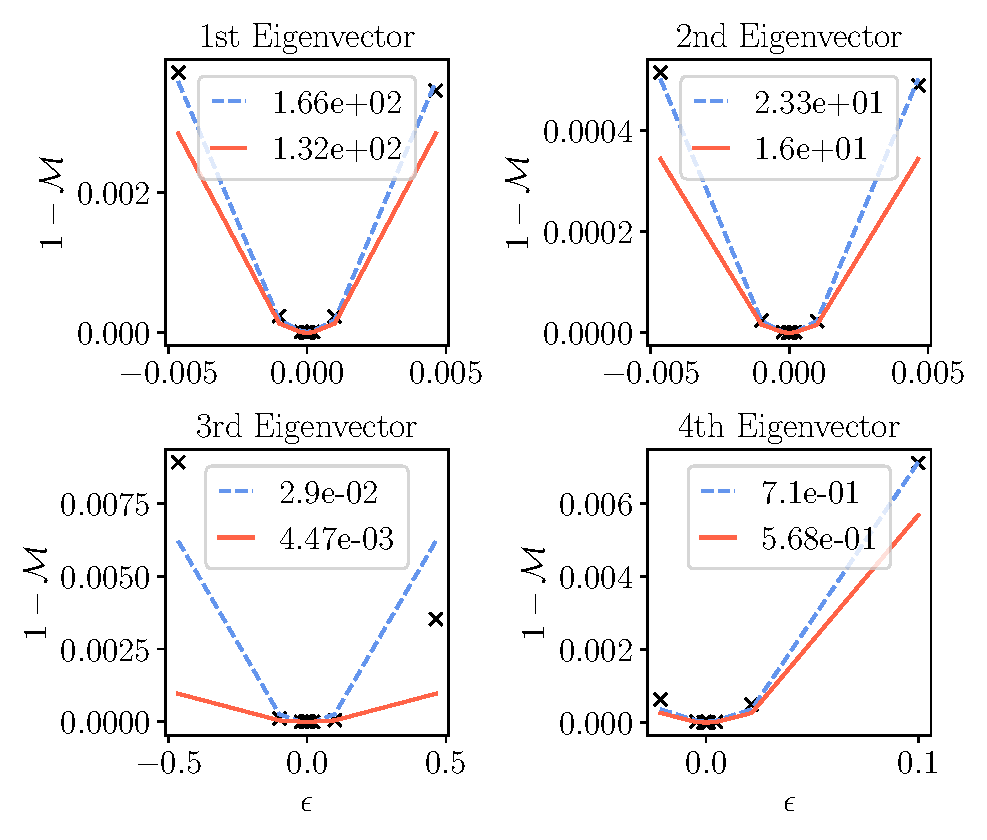
\includegraphics[scale = .52]{parabolae}
	\caption{For each eigenvector of the metric, we compute the empirical relation between the mis-match $1-\mathcal{M}$ and the distance $\epsilon$ of points along the eigenvector direction. The solid line shows the relation predicted by the metric, while the dashed line shows a parabolic fit. In the legend are reported the quadratic coefficients of both lines.}
	\label{fig:parabolae}
\end{figure}

Throughout this paper, we identified the metric with the Hessian of the overlap (see Eq.~\eqref{eq:metric_expression}). While this is widely usd in the literature and has been proven to provide reliable template banks, it still has some non desiderable properties.
To show this, we compute the metric at point $\theta_0 = [20, 3., 0.7, 1.8]$ of manifold \texttt{Mq\_s1xz}, described in Sec.~\ref{sec:placing_accuracy}, and we compute its eigenvalues $\alpha^{(i)}$ and eigenvectors $v^{(i)}$ . We then compute the match $\mathcal{M}^{(i)}_\epsilon$ between $\theta_0$ and the point $\theta^{(i)}_\epsilon = \theta_0 + \epsilon v^{(i)}$, located at a distance $\epsilon$ along i-th eigenvector.
Finally, we  compute the coefficient $\alpha$ of the Taylor expansion $1 - \mathcal{M}^{(i)}_\epsilon = \alpha  \epsilon^2$.
$\alpha$ corresponds to the i-th eigenvalue and in principle, it should be close to its value.

In Fig.~\ref{fig:parabolae}, we plot the fitted relation between $1 - \mathcal{M}$ and $\epsilon$ for each eigenvector, as well as the one computed with the metric. In the legend we report the $a$ coefficient (dashed blue line) and the eigenvalue of the metric (solid orange line).
The striking feature we note in the Figure, is that the eigenvalue is consistently smaller than the fitted $a$ coefficient, sometimes by an order of magnitude.
This means that the hessian, which is computed for $\epsilon\rightarrow 0$, is not able to extrapolate the behaviour of $1 - \mathcal{M}(\epsilon)$ even at modestly large value of $\epsilon$: the metric approximation to the match loses its predictivity as a measure of distance.
The problem becomes more severe in high dimensional manifolds.
On the other hand, since the banks generated with the hessian metric show nice coverage, one may argue that the {\it volume} estimate provided by the hessian is still accurate enough for our purposes.

As a way out, we could redefine the matrix $M_{ij}(\theta)$ to a more suitable expression, departing from the Hessian.
The goodness of the metric expression may depend on the application and on the range of validity of the approximation.
The tensor field $M_{ij}(\theta)$ can be computed through an optimization problem, where we minimize the discrepancy between the two quantities in Eq.~\eqref{eq:metric_definition}, encoded into a {\it loss function}.
The loss function depends on the values of the matrix elements $M^\prime_{ij}$:
\begin{equation} \label{eq:loss_function}
	\mathcal{L}_\theta(M^\prime_{ij}) = \hspace{-4em} \int\limits_{\hspace{3em}\{d(\theta,\theta^\prime) < d_\mathrm{target}\}} \hspace{-3.8em}
		\dvol{\theta^\prime}{D}  \left[ 1 - \mathcal{M}(\theta,\theta^\prime) - M^\prime_{ij} \Delta\theta_i \Delta\theta_j \right]^2
\end{equation}
where the integration extends on a D-ball with radius $d_\mathrm{target}$ centered around $\theta$ and $d_\mathrm{target}$ is a tunable parameter, which controls the validity of the approximation.

At any given point $\theta$, the components $M_{ij}(\theta)$ of the metric are selected by minimizing the above loss:
\begin{equation} \label{eq:metric_optmization}
	M_{ij}(\theta) = \argmin_{M^\prime_{ij}}  \mathcal{L}_\theta(M^\prime_{ij})
\end{equation}
Although the minimization can be tackled with standard techniques, it requires many evaluations of Eq.~\eqref{eq:distance} and sampling from a ``complex" set such as ${\{d(\theta,\theta^\prime) < d_\mathrm{target}\}}$: in most cases this may prove unfeasible.
Future work may try to tackle this optimization problem finding a solution at a feasible computational cost: this may be beneficial to many data analysis applications, such as template placement and Fisher information matrix studies.
A number of alternative metric expression, coming from different heuristic optimization strategies, are already available in \texttt{mbank}, although not fully validated.

	%%%%%%%%%%%%%%%%%%%%%%%%%%%%%%%%% BIBLIOGRAPHY
	\bibliography{biblio.bib}
	\bibliographystyle{ieeetr}

\end{document}



